\documentclass{article}
\usepackage[utf8]{inputenc}
\usepackage{graphicx}


\title{Lab 01- Computer Networks Basics}
\author{Matthew Belanger}
\date{\today}

\begin{document}

\maketitle

\section{Question 1}
`hostname` shows a human-readable name for the machine that the command is run on.

`hostnamectl` shows a list of different fields for the target machine and is generally more verbose.

\begin{figure}[h]
    \centering
    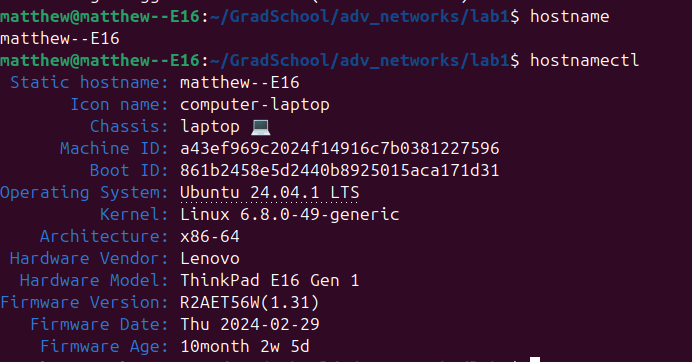
\includegraphics[width=0.8\textwidth]{./screenshots/hostname.png}
    \caption{Screenshot showing the output of `hostname` and `hostnamectl`.}
    \label{fig:hostname}
\end{figure}

\section{Question 2}
Firefox is associated with 6 ports on my VM.

\begin{figure}[h]
    \centering
    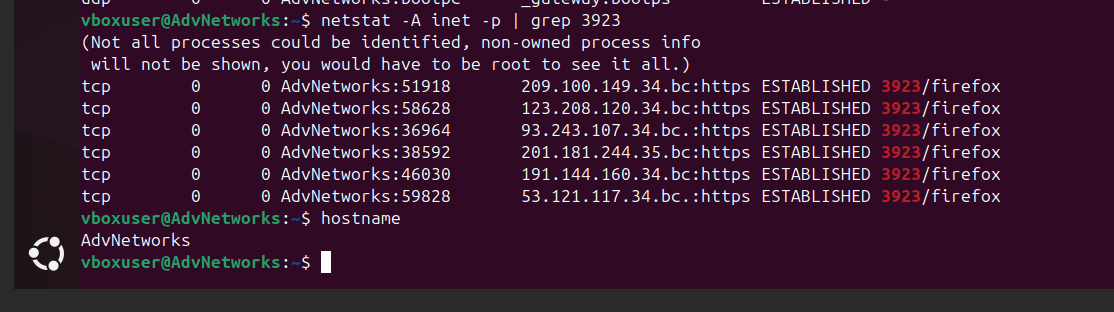
\includegraphics[width=0.6\textwidth]{./screenshots/firefox.png}
    \caption{Ports associated with Firefox connected to https://www.uwindsor.ca.}
    \label{fig:firefox}
\end{figure}

\section{Question 3}
This command displays information about my network interfaces. I can see on my machine that I have a loopback interface called `lo` and a standard interface. I can see its MAC address as well as some IP information

\begin{figure}[h]
    \centering
    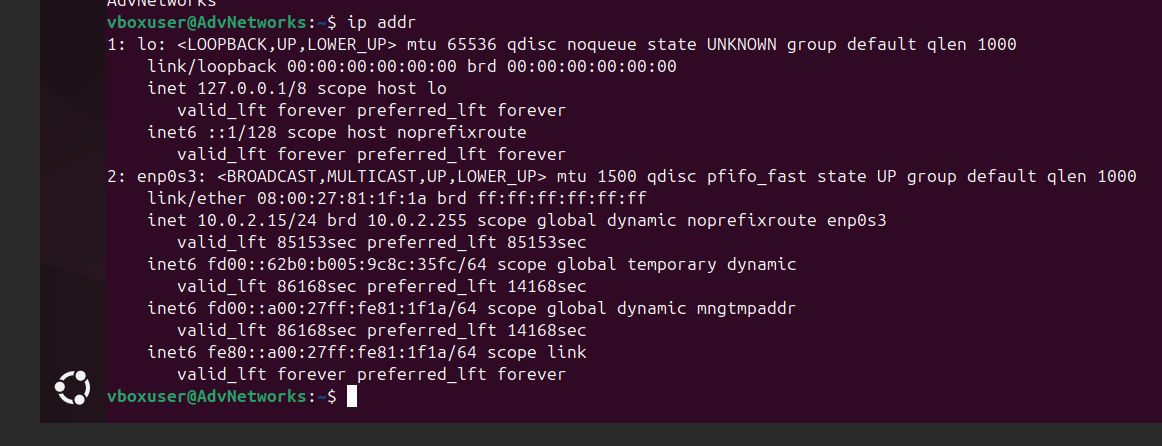
\includegraphics[width=0.6\textwidth]{./screenshots/ipaddr.png}
    \caption{Output of `ipaddr` call.}
    \label{fig:ipaddr}
\end{figure}

\section{Question 4}
See Below:

\begin{figure}[h]
    \centering
    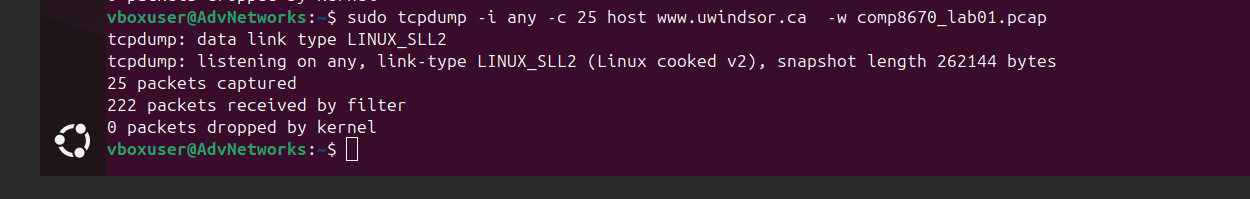
\includegraphics[width=1\textwidth]{./screenshots/tcpdump.png}
    \caption{Packet Capture}
    \label{fig:tcpdump}
\end{figure}

\section{Question 5}
Yes I did it.

\end{document}
